\documentclass[10pt,a4paper]{article}
\usepackage[utf8]{inputenc}
\usepackage{amsmath}
\usepackage{amsfonts}
\usepackage{amssymb}
\usepackage{graphicx}
\usepackage{enumerate}
\begin{document}

\section{Set Theory}

To demystify mathematics consider
\begin{enumerate}[(i)]
\item What is a theorem?
\item What is a proof?
\end{enumerate}
What if we don't know the answer?

To begin we need
\begin{enumerate}[(a)]
\item an example(s)
\item a nearly related concept
\end{enumerate}


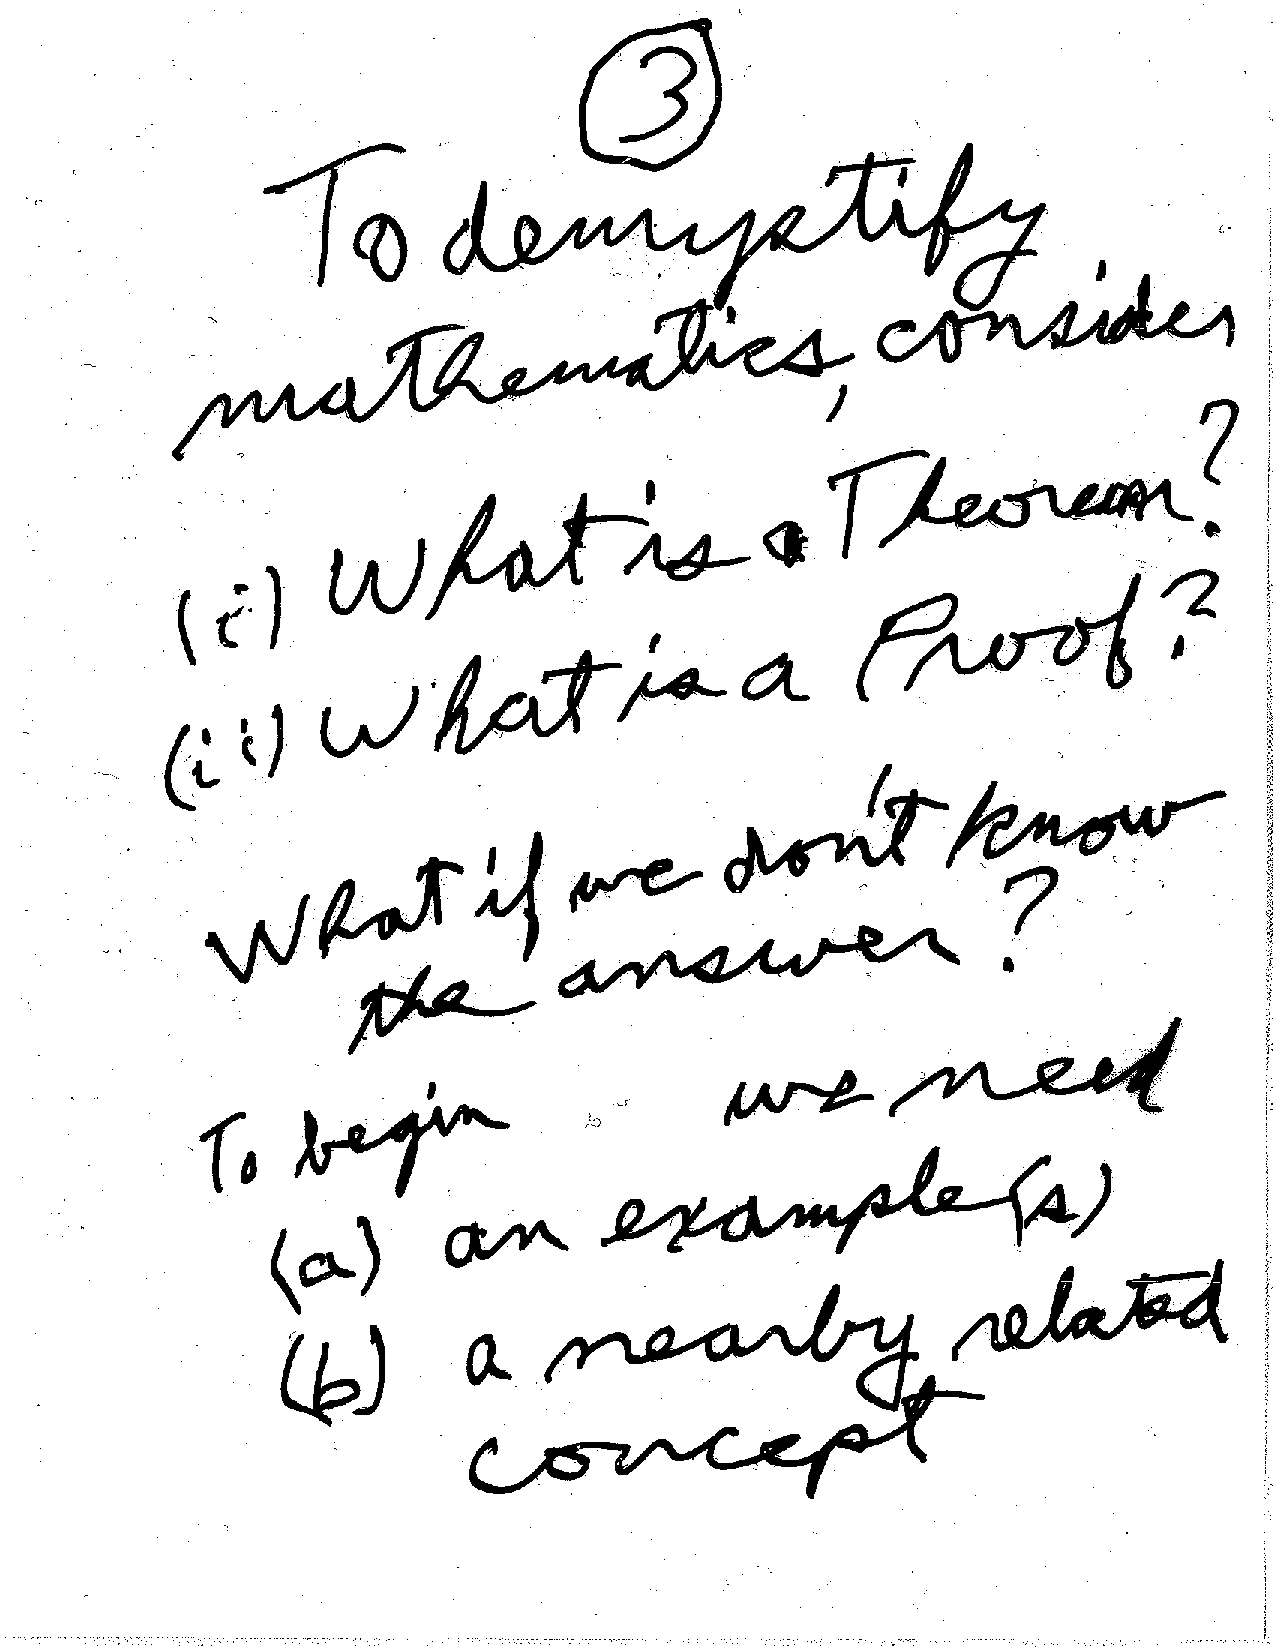
\includegraphics[scale=.5]{Pages/ST_3}

\newpage

Related Concept: Greek Syllogism

\underline{example:}
\begin{enumerate}
\item All men are mortal.
\item Socrates is a man.
\item Therefore, Socrates must die. 
\end{enumerate}

To analyze, recast in set theoretic terms via Venn Diagram.

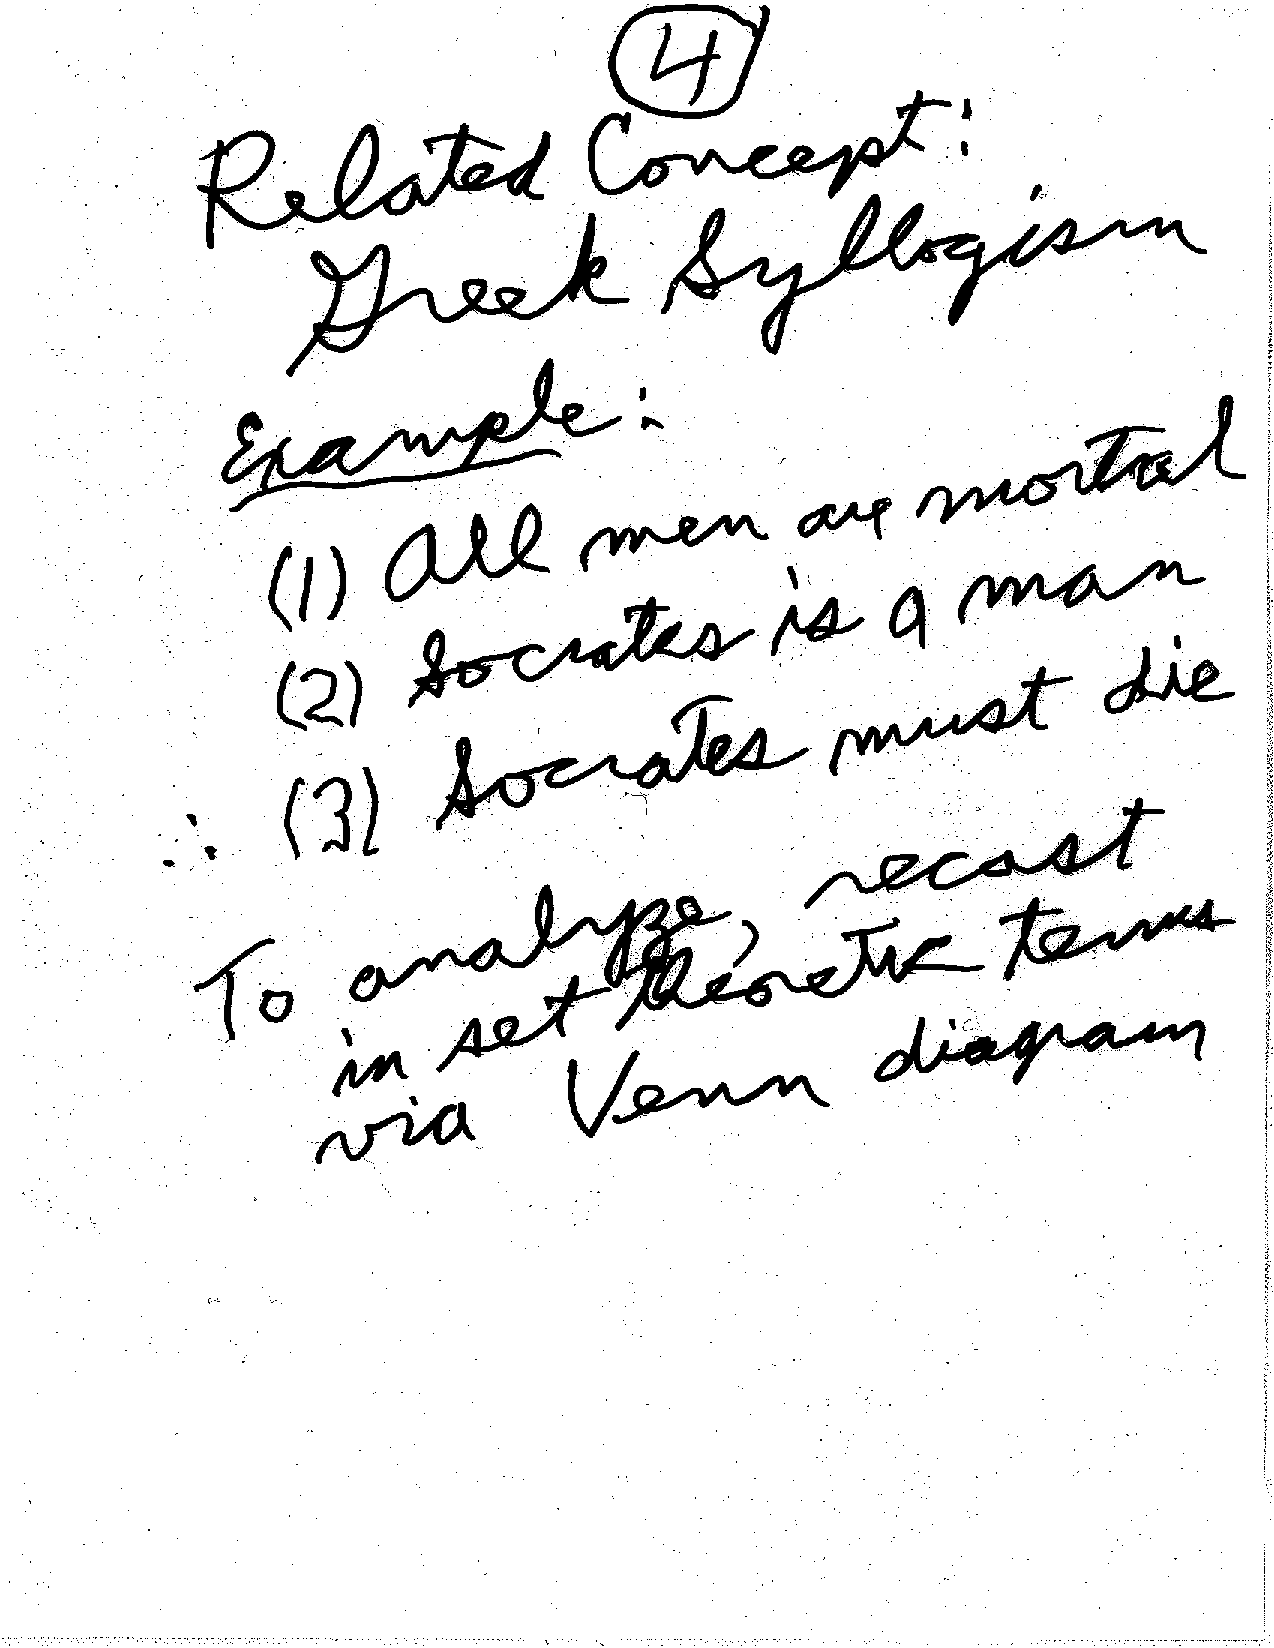
\includegraphics[scale=.5]{Pages/ST_4}

\newpage

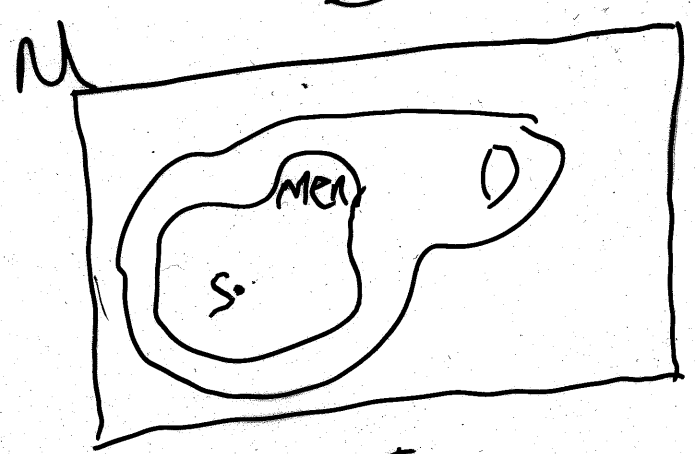
\includegraphics[scale=.2]{Pages/ST_5_im1}

$S$: Socrates\\
$M$: Set of Men\\
$D$: Things that will die\\
$\mathcal{U}$: Things on Earth

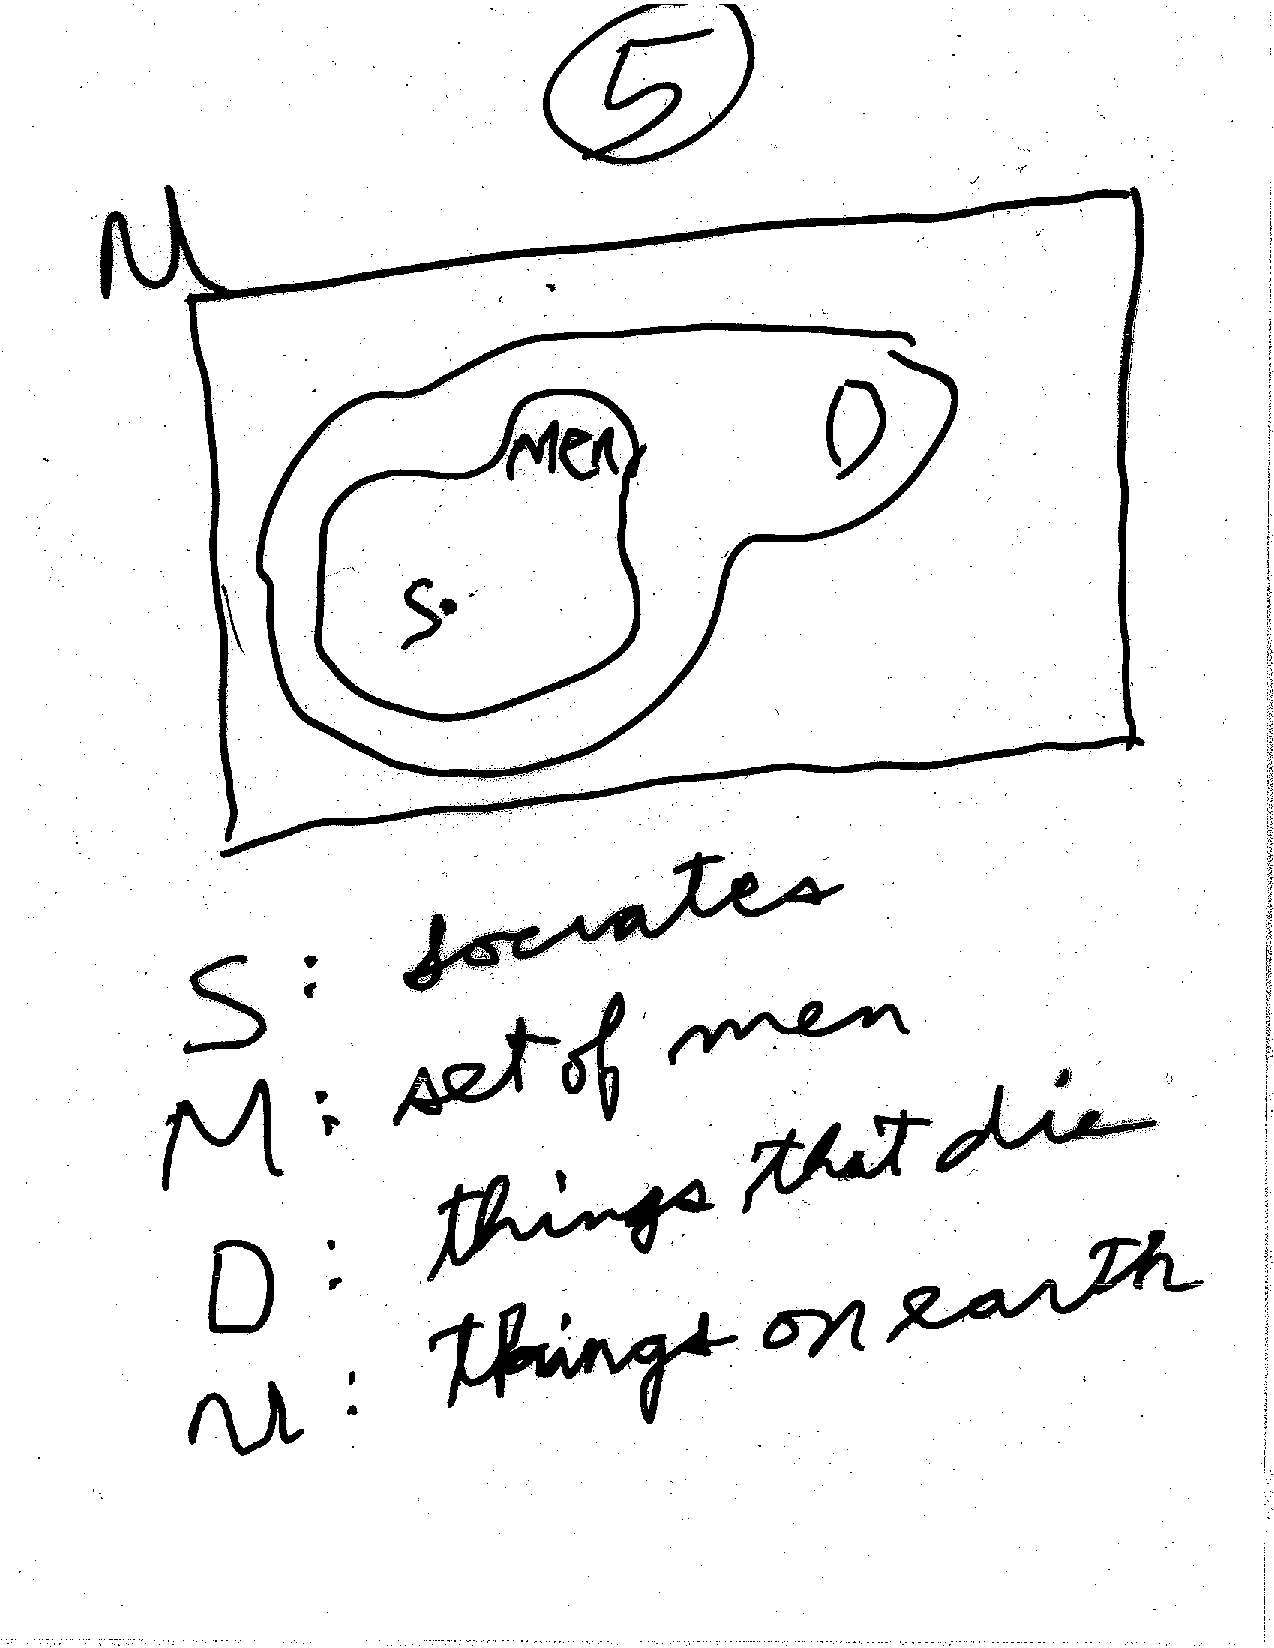
\includegraphics[scale=.5]{Pages/ST_5} 



%Zack: Pages 6,7,8,19,20

%Jack: 21, 9, 10, 11

%Koka: Pages 13, 13A, 22 ,22A, 22B


\section{Generate $\mathbb{N}$}


%Ruth: Pages L4A-L4G




\section{From $\mathbb{Z}$ to $\mathbb{R}$ via ordering}
%Jazz: ZR1-ZR5

%Kyler: ZR6 - ZR10

%Preethika: ZR11-ZR14


\section{Sequence and Limits}

%Aaron: First 2 pages and 48-50

%Hamza: 51-52B

\section{Limit and Convergence}

%Joe: 50-51

%Quinten: 52-53

%Farishta: 53A-54A

\section{Infinite Series}

%Sukhreet: IS1 - IS 7

%Matthew: IS8 - IS15

%Will: IS16 - IS23

%Rebecca: IS24 - IS32

%Maady: IS33 - IS42

\section{Metric Spaces Part 1}

%Travis: M1 - M5

%Jerome: M6- M10



\section{Metric Spaces Part 2}


%Bryant: M1-M7

%Reshma: M8-M14
\newpage
\Large
\center \underline{Reformulation} {\bf M8} \underline{Convergence}
\begin{flushleft}
We can use collections of points to determine whether a sequence converges. \\Let $D_r(x) = \{y\in M = d(x,y) <r\}$\\
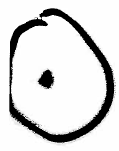
\includegraphics[scale=.5]{Pages/MS_8_Im}
\\Fact: $$\lim_{n\rightarrow \infty} x_n = x $$ if and only if  
$\forall \varepsilon > 0 \exists N_{\varepsilon} < \infty: x_n \in D_{\varepsilon}(x)$\\for all n $\geqslant N_{\varepsilon}$
$D_r(x)$ is called the open disk (ball, sphere) of radius $r$ about $x$.\\
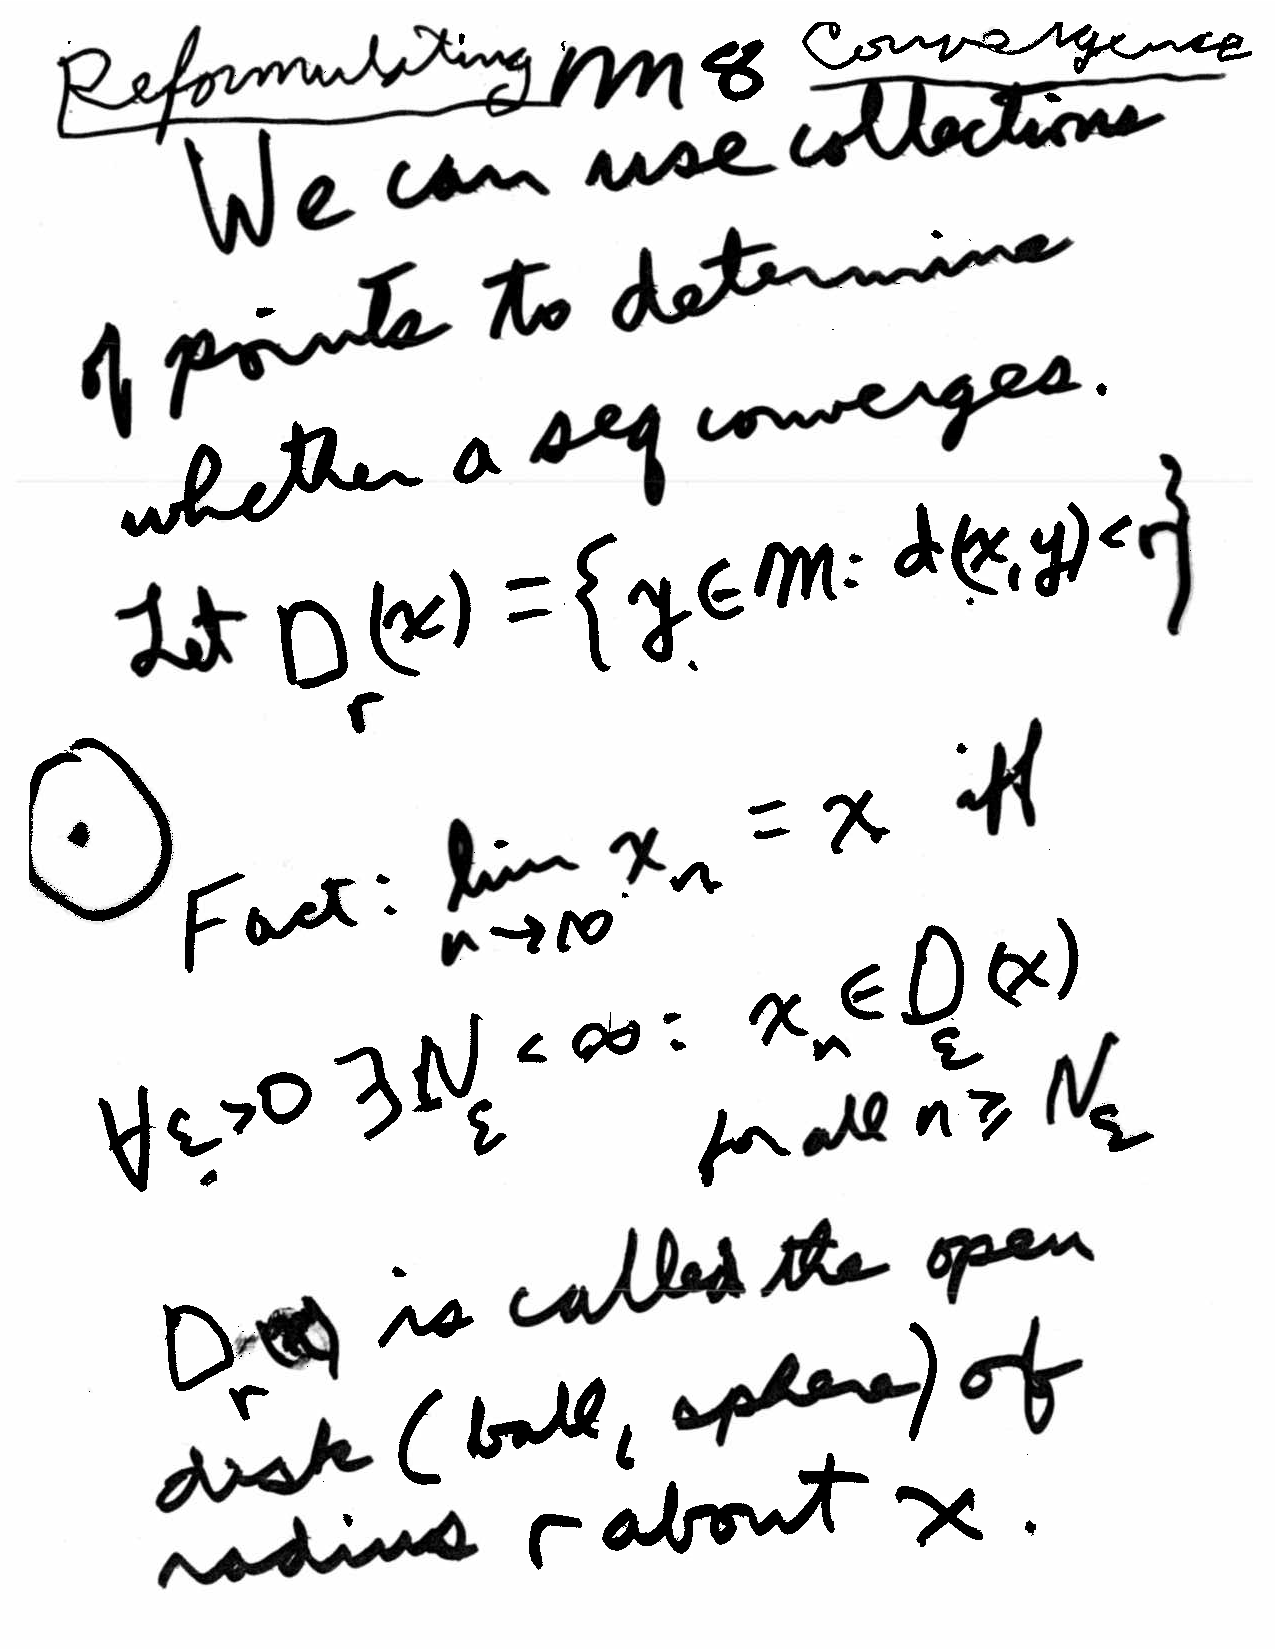
\includegraphics[scale=.4]{Pages/MS_8}
\newpage

Rudin calls it an r neighborhood of $x$, or just a neighborhood. Are there more general families of sets of points in a metric space ($m, d$) that could be used to determine convergence of sequences regardless of the particular sequence or its limit?
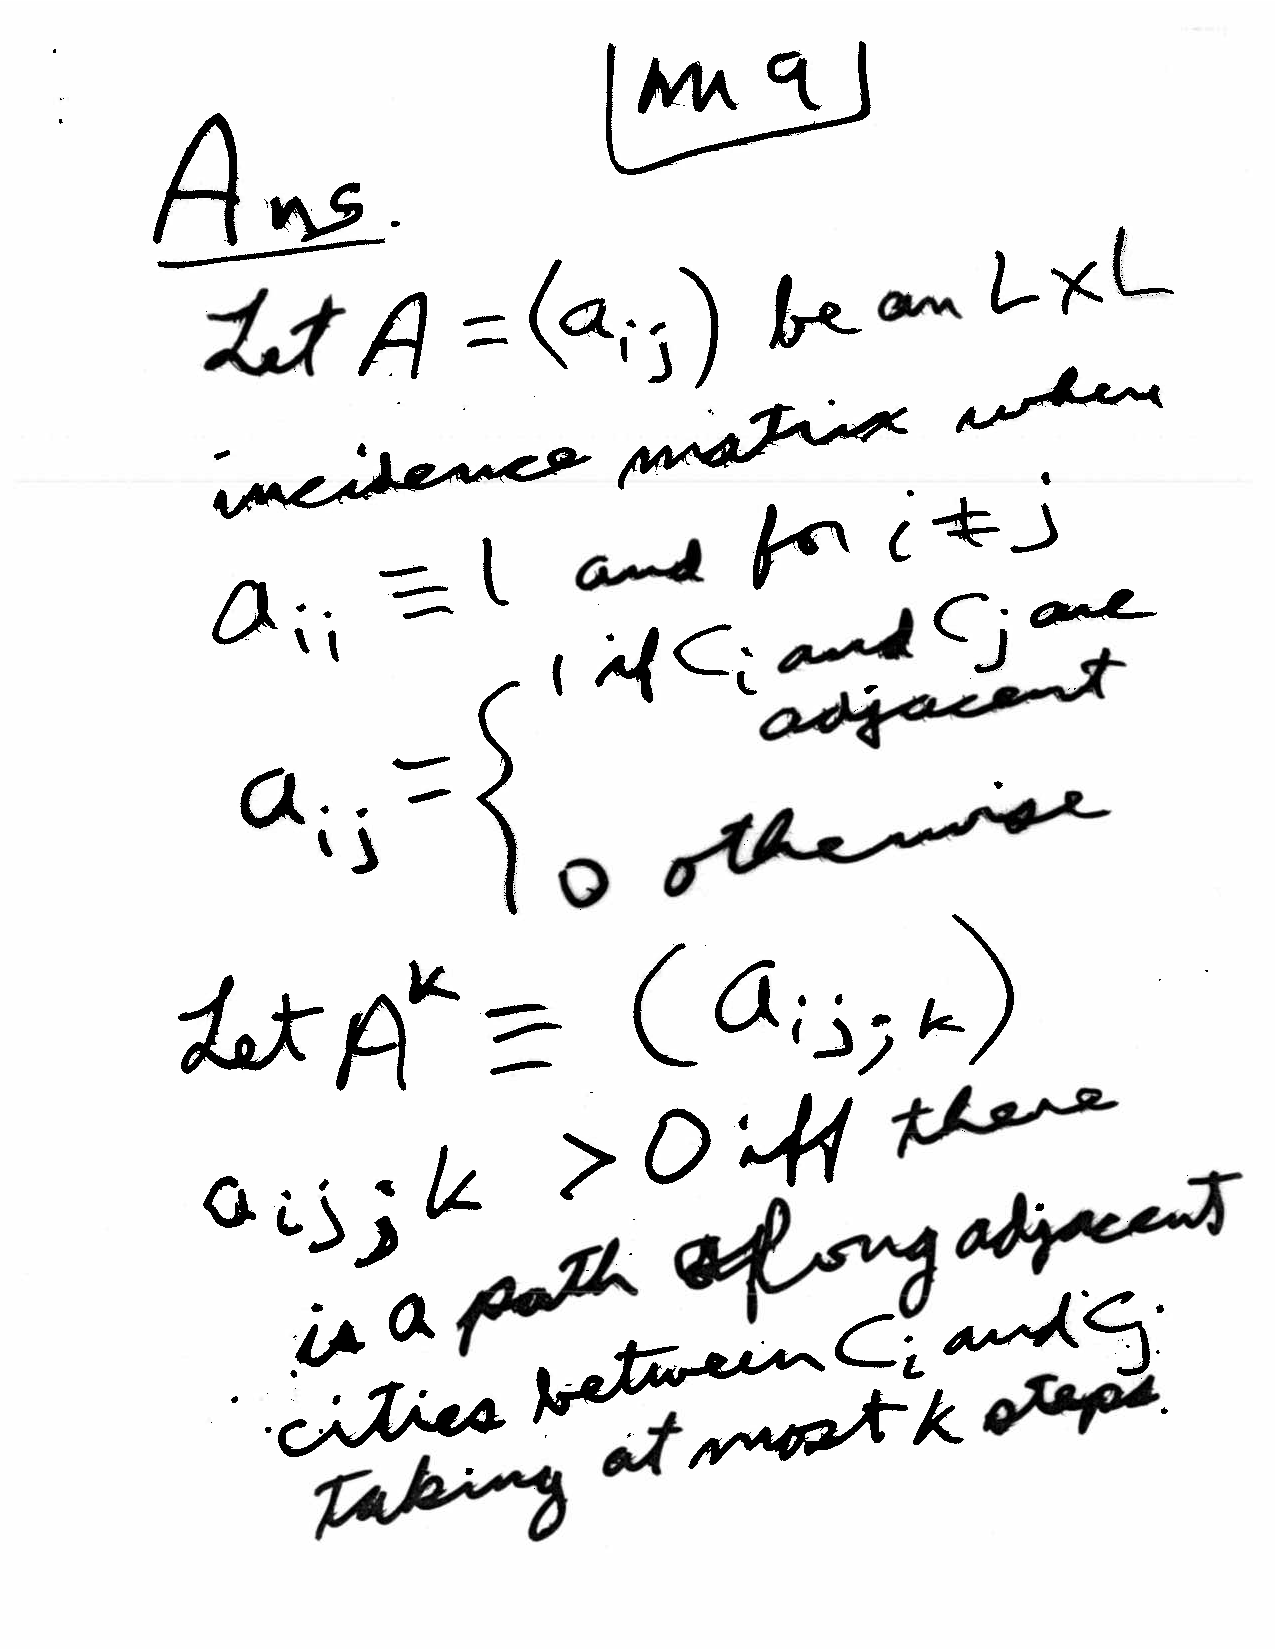
\includegraphics[scale=.5]{Pages/MS_9}
\newpage

For each point x of such a set $\mathcal{O}$, if $x_n \rightarrow x$ there must be an $\varepsilon_o > 0$ such that for all 0 $< \varepsilon < \varepsilon_o$ \\ $D_{\varepsilon}(x)\subseteq \mathcal{O}$ so that $X_n \in \mathcal{O}$ for all n sufficiently large.\\ \underline{Definition} $\mathcal{O}\subseteq \mathcal{M}$ is ($m,d$) an \underline{open set} in $\mathcal{M}$ if and only if $\forall x \in \mathcal{O } \exists E > 0$ such that $D_\varepsilon(X) \subseteq \mathcal{O}$\\
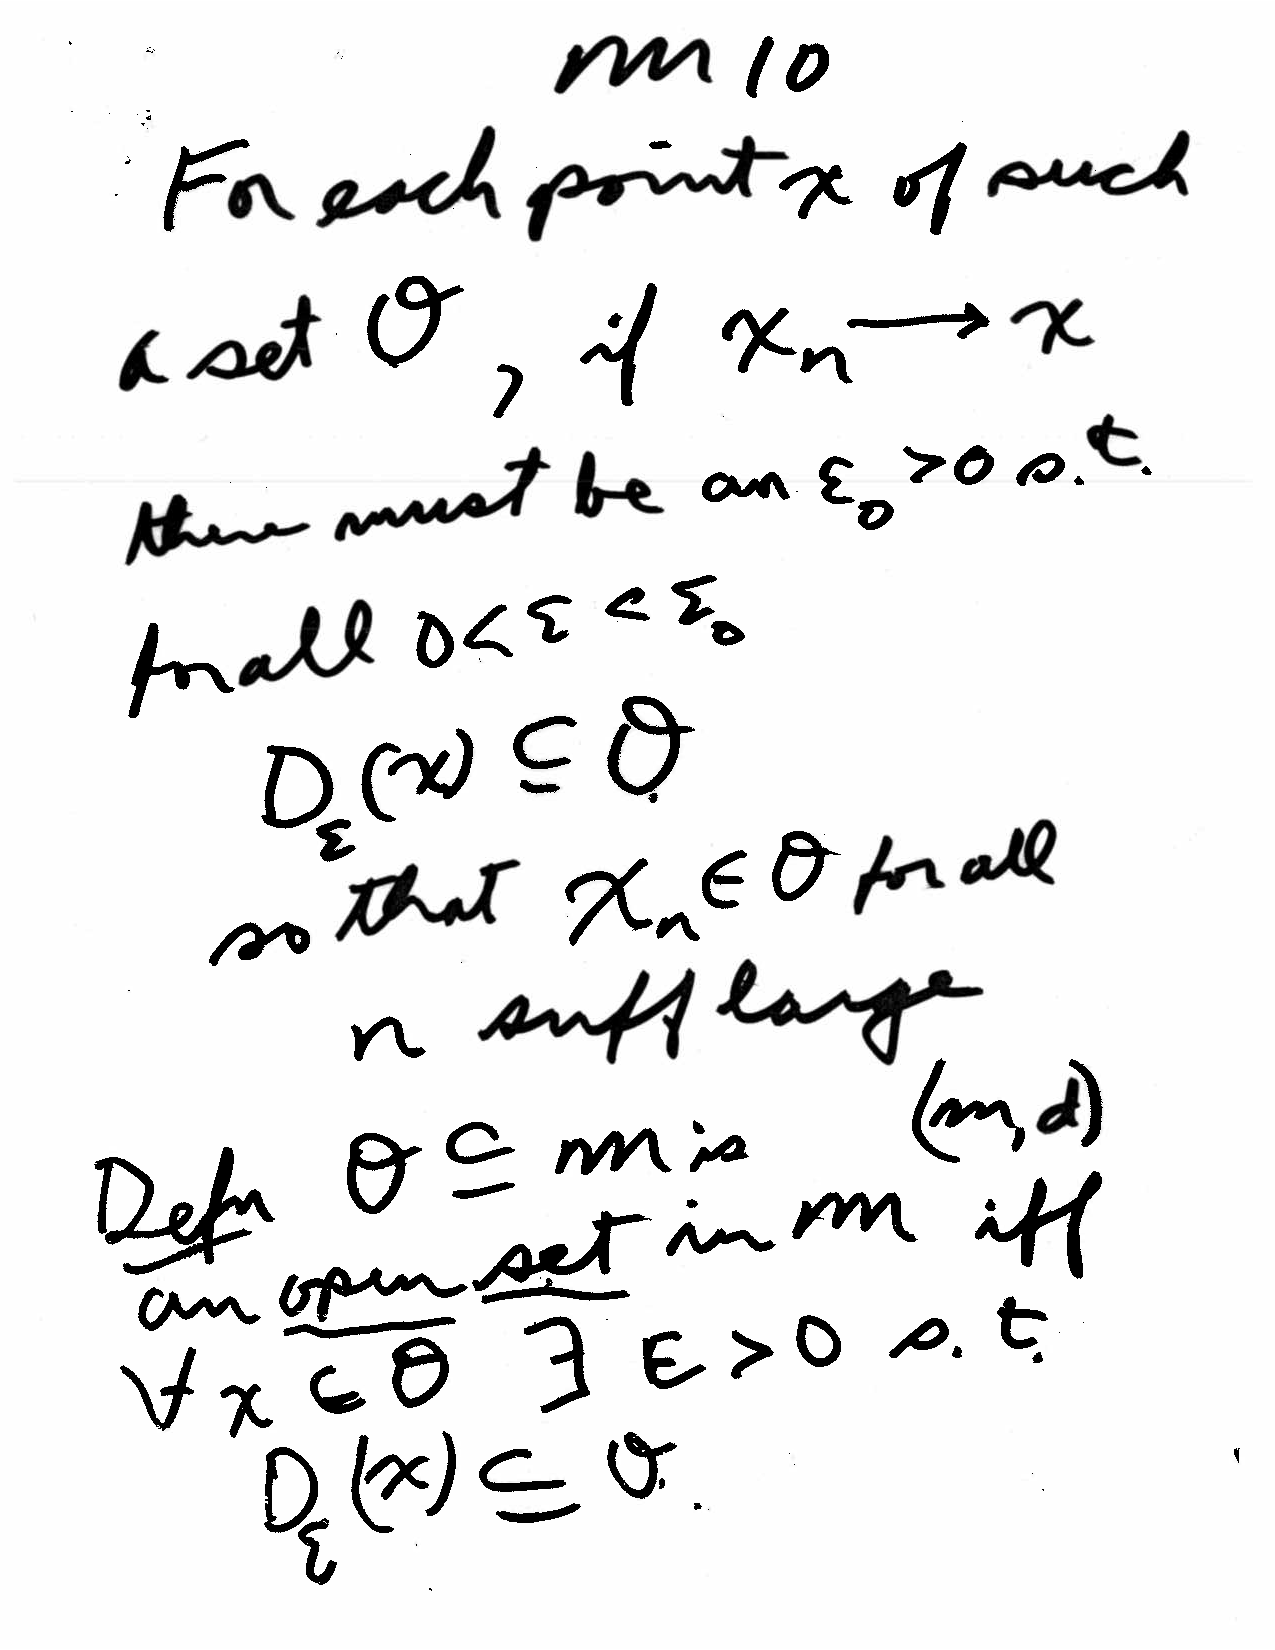
\includegraphics[scale=.5]{Pages/MS_10}
\newpage

For all metric spaces ($m,d$), $ \varnothing, \mathcal{M}$ and $D_r(x)$ for $x \in \mathcal{M}$ and $r \geq O$ are always open sets.\\
\center{ Properties of Open Sets}\\
\end{flushleft}
\begin{flushleft}
\begin{description}
  \item[(i)] Definition \{$\mathcal{O}_\alpha:\alpha \in J$\} are open in $\mathcal{M}$ so is $$ \bigcup_{\alpha \in J} \mathcal{O}_\alpha $$
  \item[(ii)] Definition $\mathcal{O}, \cdots, \mathcal{O}_n$ are open in $\mathcal{M}$ so is $$\bigcap^n_{j=1} \mathcal{O}_j$$ (Arbitrary unions of open sets are open. Intersections of finitely many open sets are open.) 
\end{description}
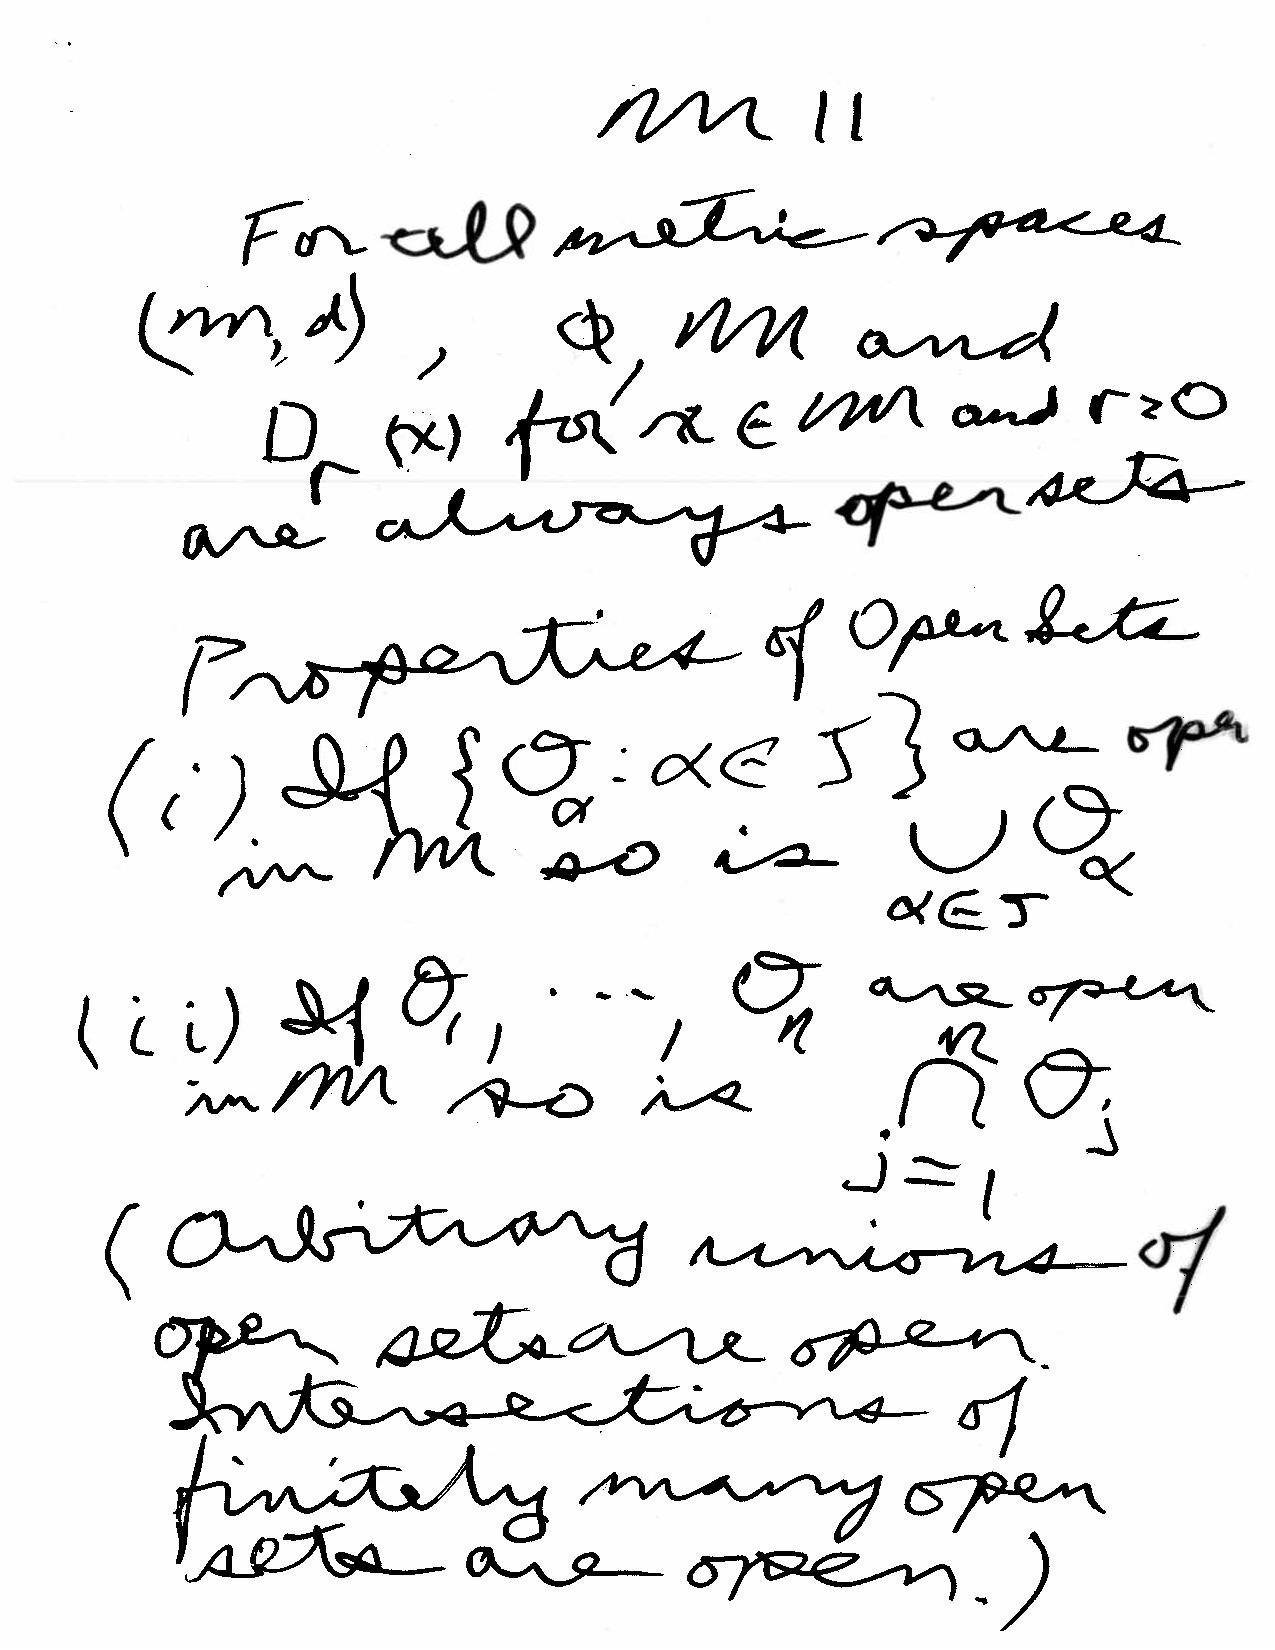
\includegraphics[scale=.4]{Pages/MS_11}
\newpage  
Definition $x$ is an \underline{interior point} of A $\subseteq M$ if an only if $\exists \varepsilon > 0: D_\varepsilon(x) \subseteq A $\\ $A^O =$ \{All interior points of A \} \underline{Fact: }$A^O$ is the largest open subset of $A$.\\ \underline{Definition} $x$ is a limit  point of $A\subseteq M$ if and only if $\forall \varepsilon>0 |D_\varepsilon(x) \bigcap A| \geq 2$ if an only if $\forall \varepsilon>0 (D_\varepsilon(x)\backslash \{x\}$)$\bigcap A \neq \emptyset$
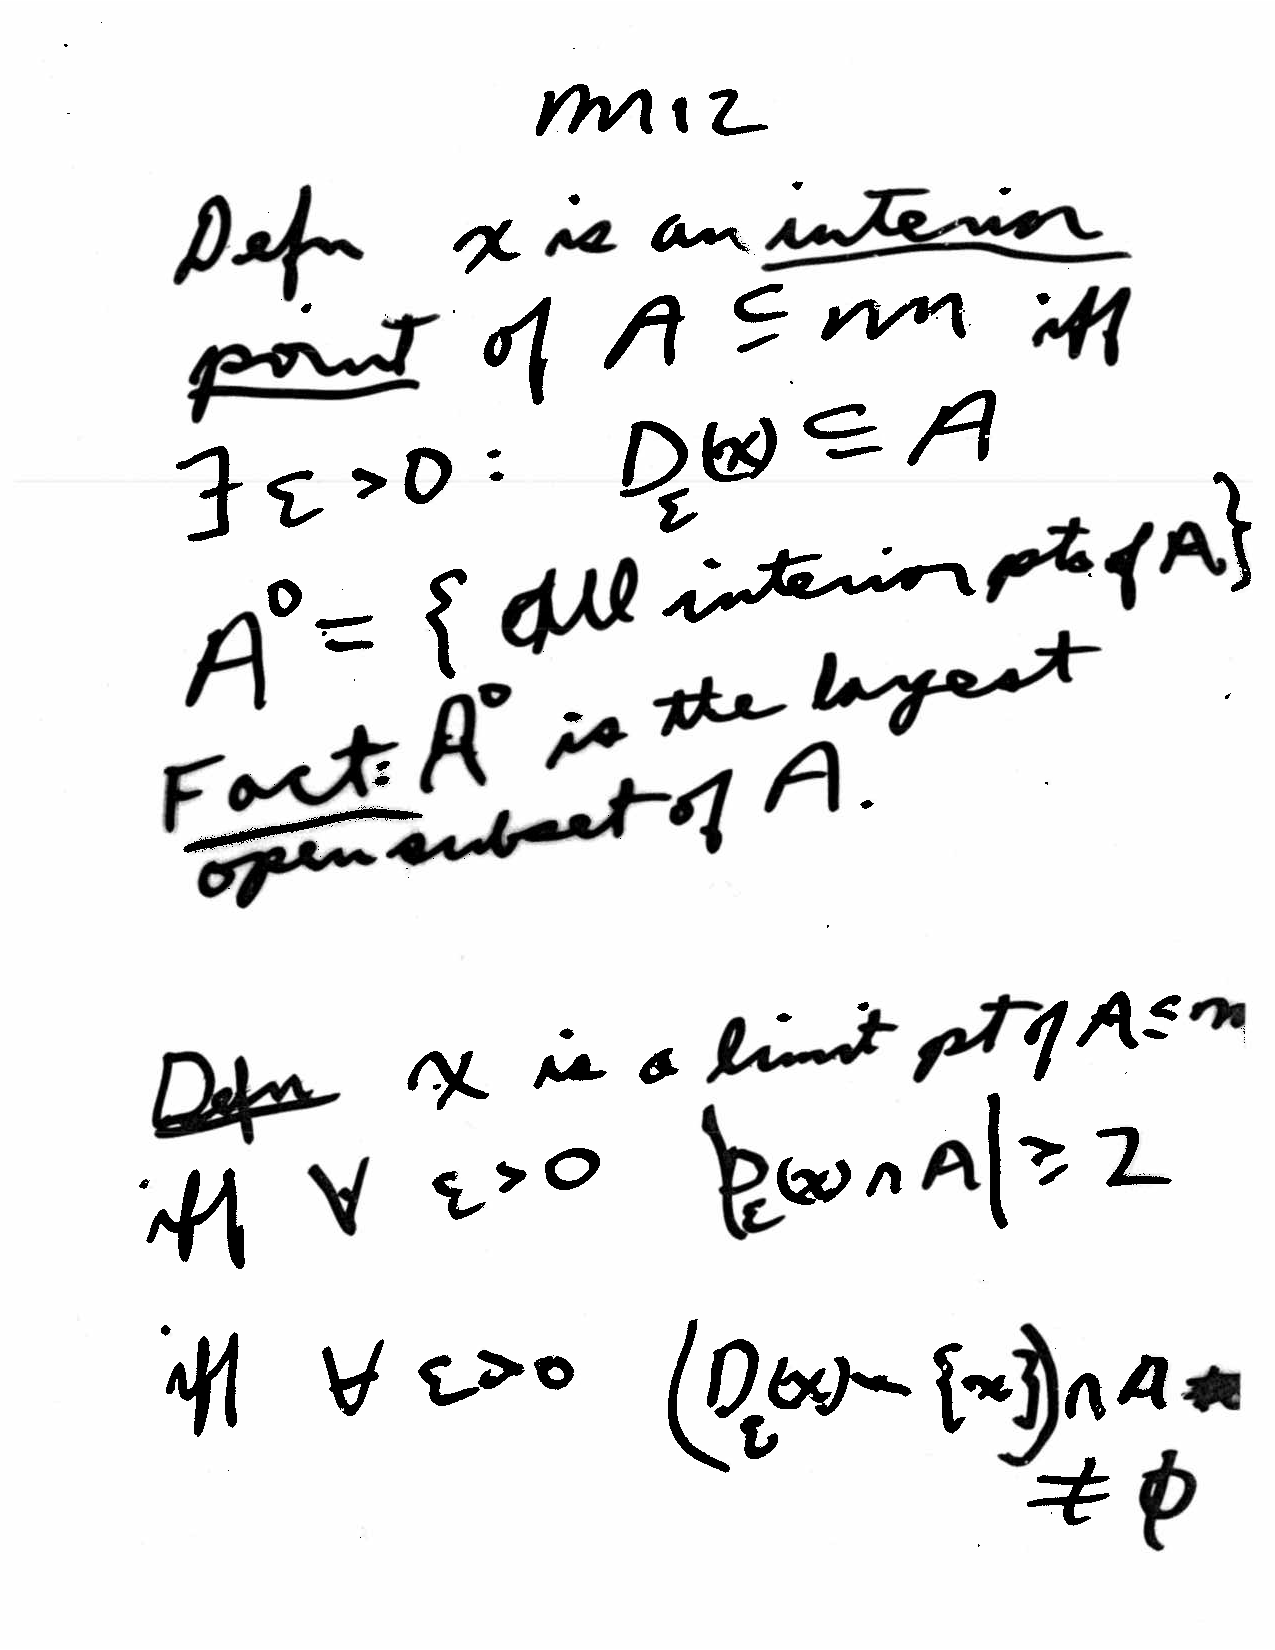
\includegraphics[scale=.5]{Pages/MS_12}
\newpage
\underline{Proposition} $x$ is a limit point of $A$ if and only if $\exists$ sequence of distinct points of $A$ that converges to $x$. \\ \underline{Definition} $F \subseteq M$ is \underline{closed} if and only if every limit point of $F$ belongs to $F$.
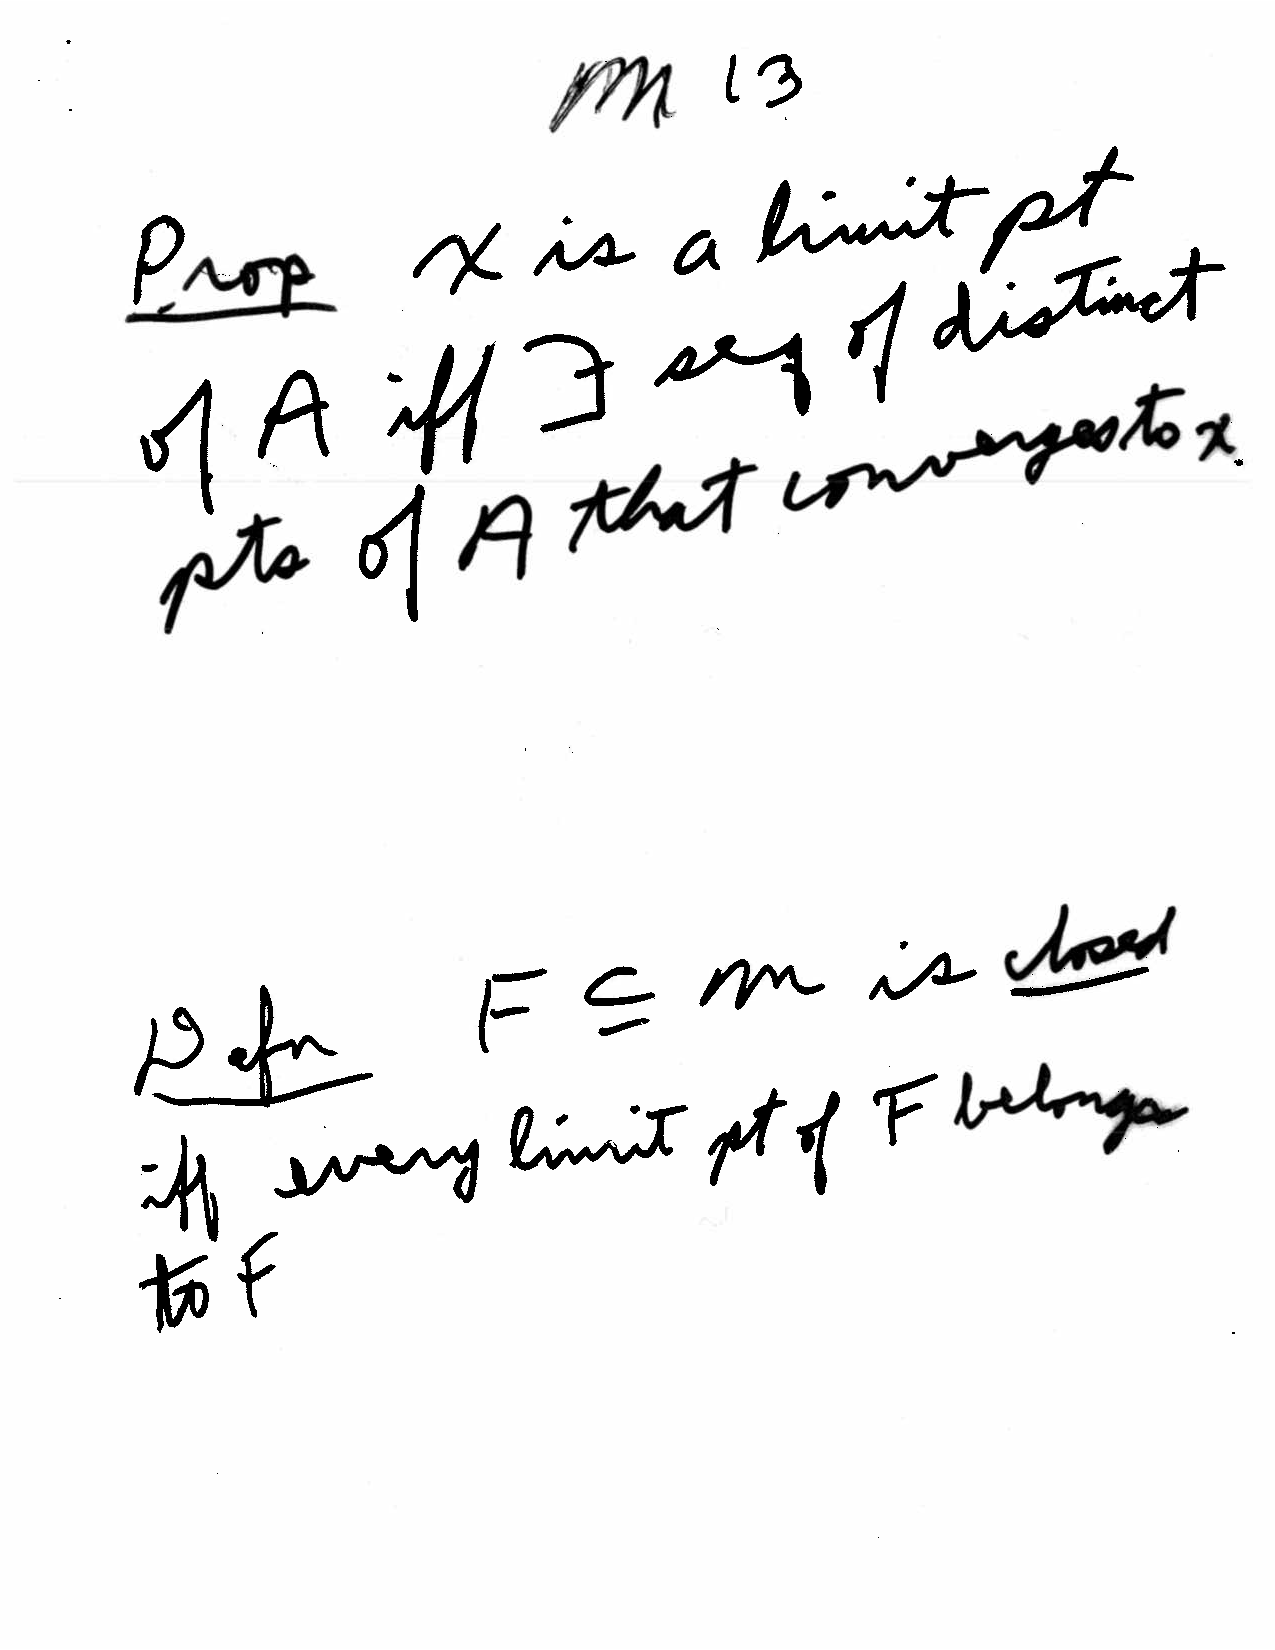
\includegraphics[scale=.5]{Pages/MS_13}
\newpage
Examples of closed sets in $\mathbb{R}^1$ and $\mathbb{R}^2$

$\emptyset$ and $M$ are always closed space $F_j$ and $F_{\alpha}$ are closed in $M$.
\begin{description}
\item[i] if $F_1, \cdots, F_n$ are closed, so is $$ \bigcup^n_{j=1} F_j$$
\item[ii] if $F_\alpha$ is closed for $\alpha \in J$ so is $$\bigcap_{\alpha \in J} F_\alpha$$
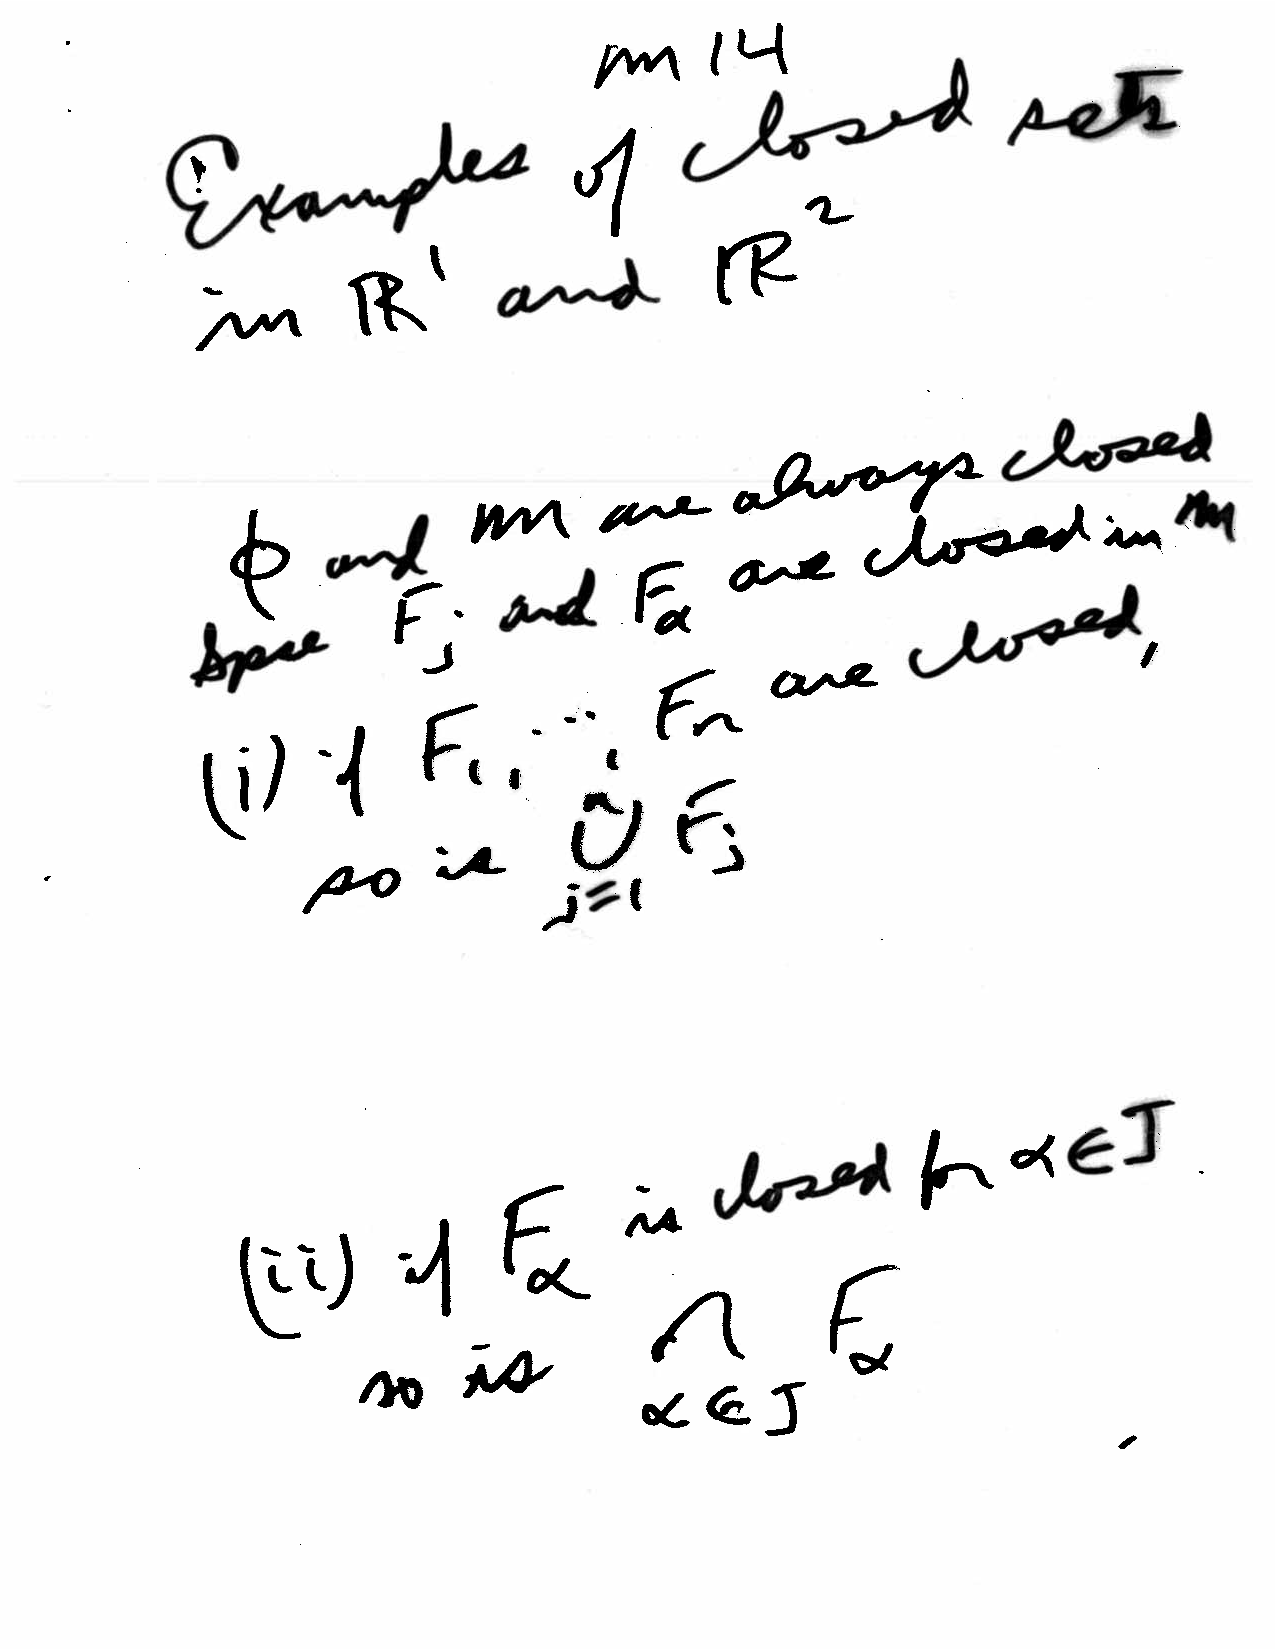
\includegraphics[scale=.5]{Pages/MS_14}
\end{description}
\newpage
How should we define $\partial E$, the boundary of a set E?

Certainly $\partial E \subseteq \overline{E}$ since the boundary could involve points of $E$ and points infinitesimally close to points of $E$. However, $\partial E = \partial E^c$ so $\partial E \subseteq \overline{(E^c)}$
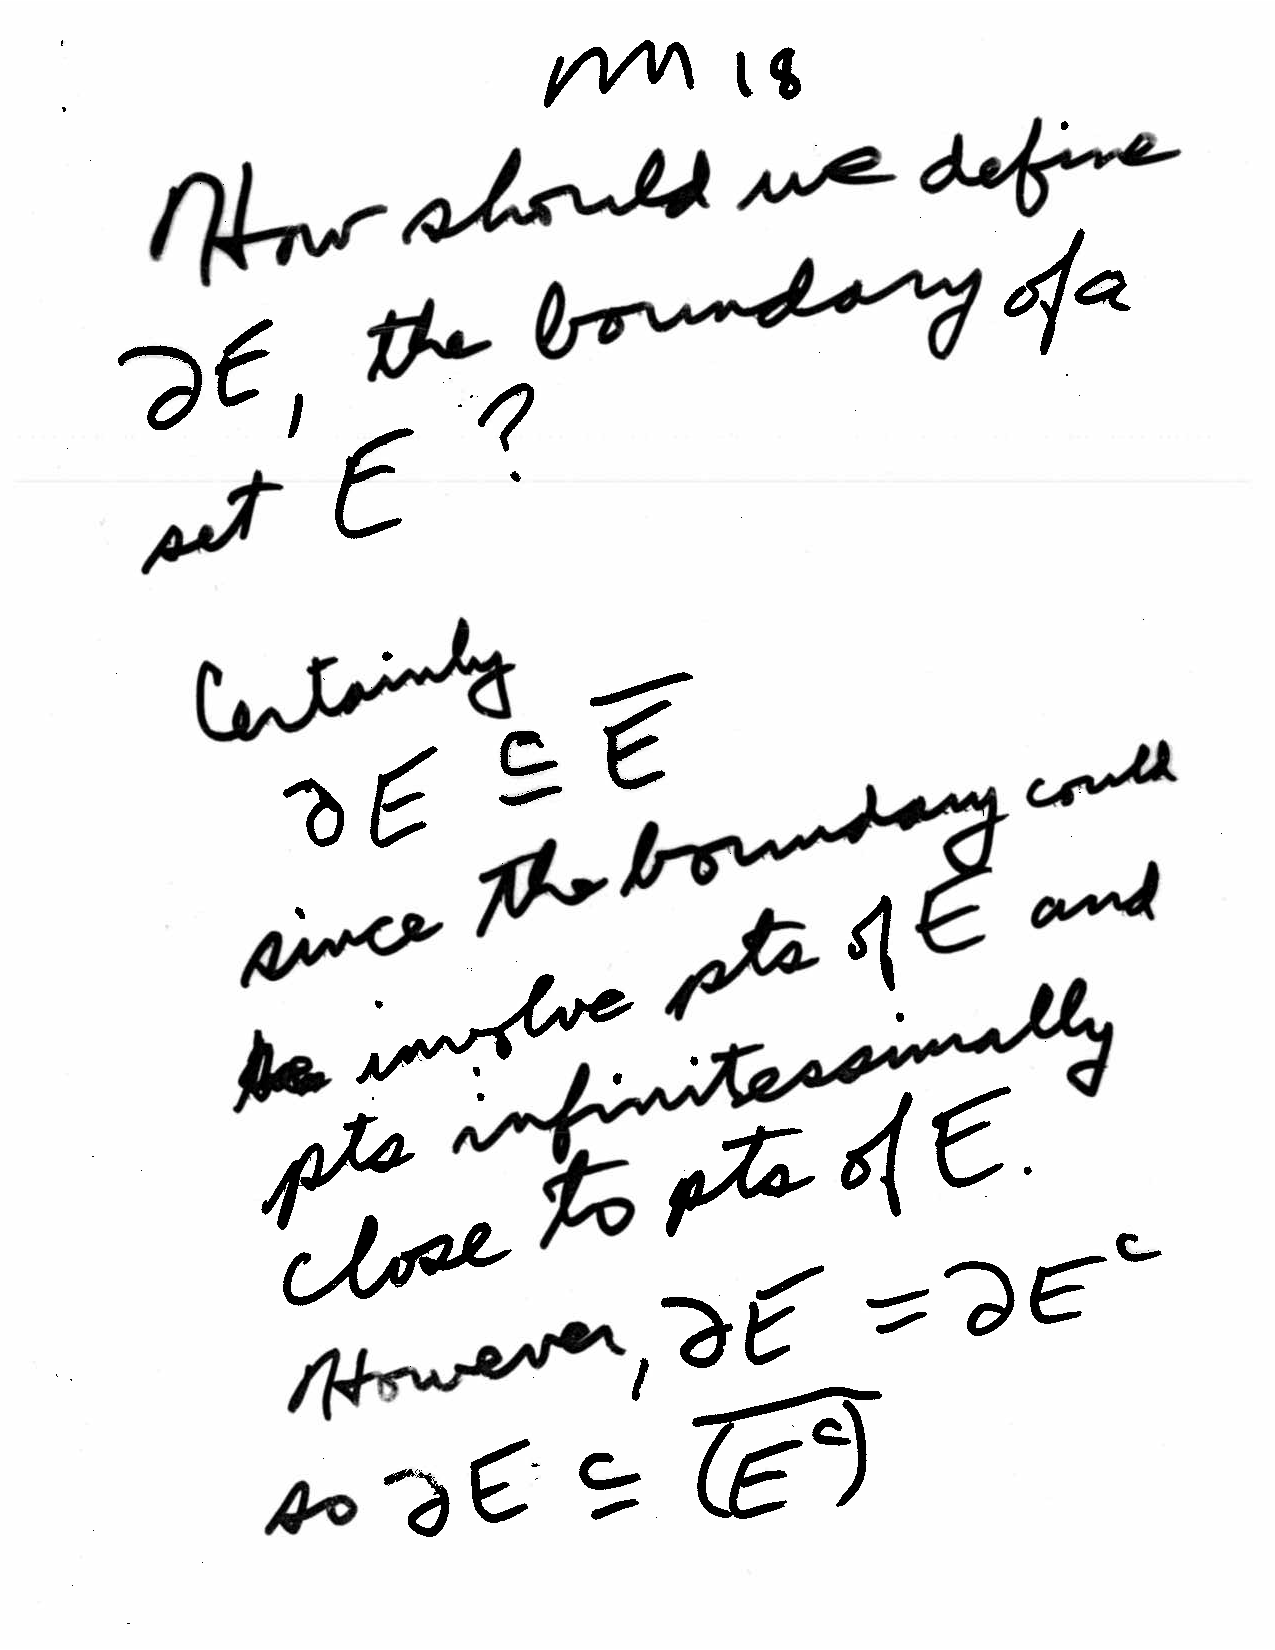
\includegraphics[scale=.5]{Pages/MS_18}

\newpage
\underline{Definition} $\partial E = \overline{E} \bigcap \overline{(E^c)}$\\ $\partial E$ is called the \underline{boundary} of the set $E$. 

Can $\partial E \varsupsetneqq E$?

Fact: $\overline{E} = E \bigcup (\partial E)$
\line(1,0){330} \\
Suppose $E \subseteq F \subseteq M (m,d)$\\
\underline{Definition} $E$ is dense in F\\ if and only if $\overline{E} \supseteq F$\\ if and only if every point of $F$ in $E \bigcap$ is a limit point of $E$\\ if an only if $\forall x \in F \exists x_n \in$ such that $x_n \rightarrow x$\\ Then $E$ is dense in $F$
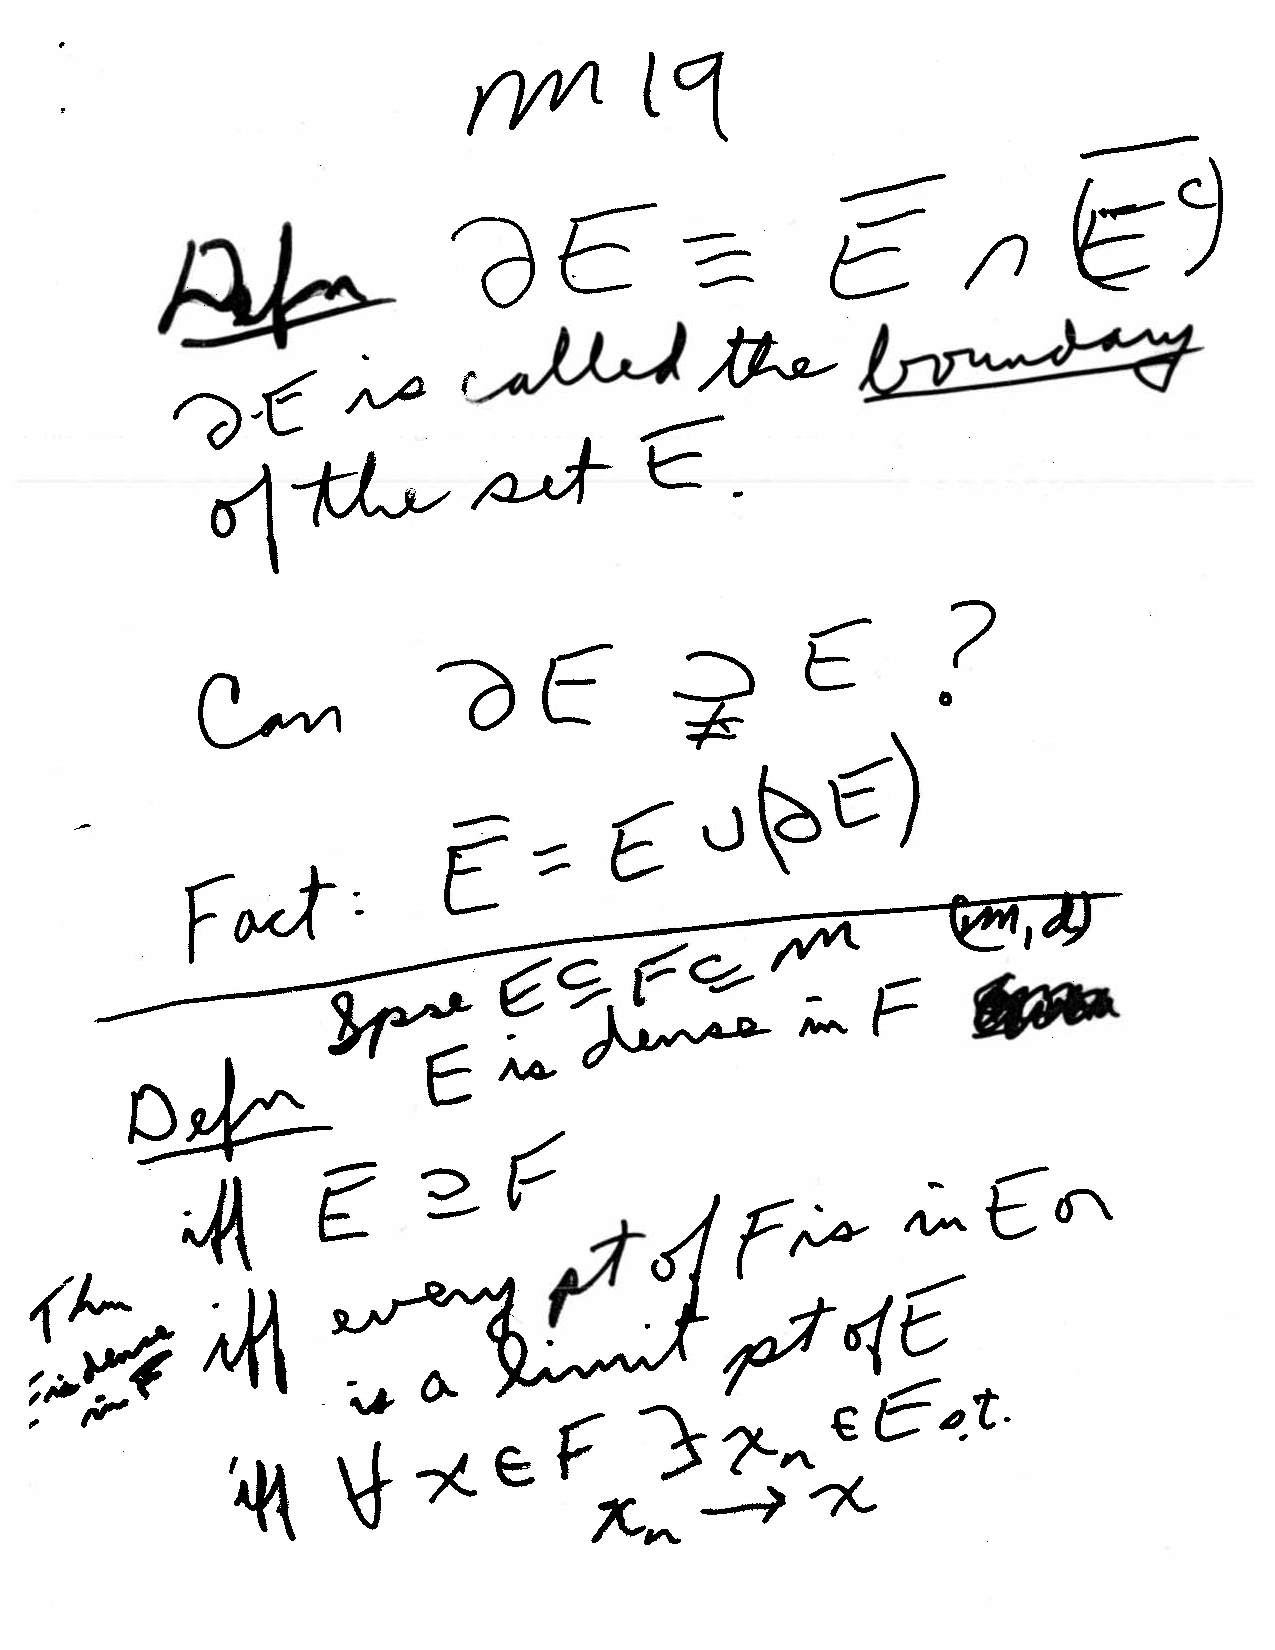
\includegraphics[scale=.4]{Pages/MS_19}

\end{flushleft}
%Ethan: M15-M21





\end{document}